\documentclass[10pt]{beamer}

\usepackage[bahasa]{babel}

\usetheme{metropolis}           % Use metropolis theme

\title{Medan Elektromagnetik}

\subtitle{Kerapatan Fluks Listrik, Hukum Gauss, dan Divergensi}

\date{\today}

\author{Mifta Nur Farid, S.T., M.T.}

\institute{Teknik Elektro - Institut Teknologi Kalimantan \\ Karang Joang, Balikpapan, Indonesia}

\begin{document}

\maketitle

\section{Kerapatan Fluks Listrik}

\begin{frame}{Kerapatan Fluks Listrik}
    \begin{columns}[T,onlytextwidth]
        \column{0.5\textwidth}
        
        \begin{itemize}
            \item Percobaan Faraday menunjukkan adanya "\emph{displacement}" atau perpindahan muatan dari bola bagian dalam ke bola bagian luar yang independen terhadap medium, yang disebut dengan \emph{displacement}, \emph{displacement flux}, atau \emph{electric flux}.
            
            $$ \psi = Q$$
            
            dimada $\psi$ adalah fluks listrik (\emph{electric flux}) dan $Q$ adalah total muatan di bola dalam atau \emph{inner sphere}.
        \end{itemize}
            
        \column{0.5\textwidth}
        \begin{figure}
            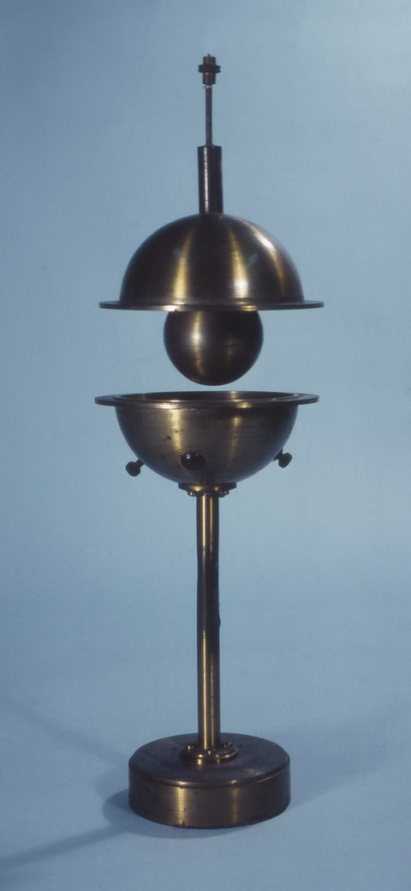
\includegraphics[width=0.5\linewidth]{chap03/faraday-exp.jpg}
            \caption{Percobaan Faraday}
          \end{figure}
    \end{columns}
\end{frame}

\begin{frame}{Kerapatan Fluks Listrik}
    \begin{columns}[T,onlytextwidth]
        \column{0.6\textwidth}
        \begin{figure}
            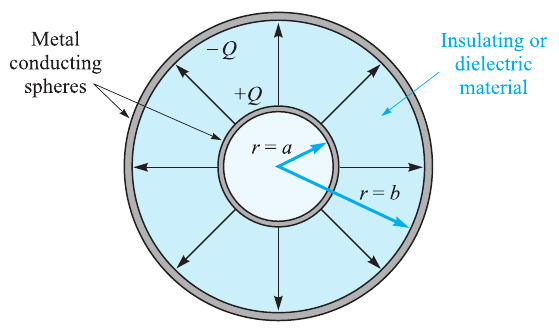
\includegraphics[width=\linewidth]{chap03/electric-flux.png}
            \caption{Fluks Listrik}
        \end{figure}

        \column{0.4\textwidth}
        \begin{itemize}
            \item Kerapatan Fluks Listrik ($\textbf{D}$) adalah fluks listrik $\psi$ yang terdistribusi uniform pada luasan $4\pi a^2~m^2$
            \item Kerapatan Fluks Listrik ($\textbf{D}$) dalam arah radial dan nilainya adalah
            \begin{equation}
                \textbf{D} = \frac{Q}{4 \pi r^2}\textbf{a}_r
            \end{equation}
            dengan $a \leq r \leq b$
        \end{itemize}
    \end{columns}
\end{frame}

\begin{frame}
    \begin{itemize}
        \item Intensitas medan listrik radial dari satu titik muatan pada ruang hampa
        $$ \textbf{E} = \frac{Q}{4 \pi \epsilon_0 r^2 }\textbf{a}_r$$
        \item Sehingga kerapatan fluks listrik pada \alert{ruang hampa},
        \begin{equation}
            \textbf{D} = \epsilon_0 \textbf{E}
        \end{equation}
        \item Untuk distribusi muatan volume pada ruang hampa, secara umum persamaannya adalah
        \begin{equation}
            \textbf{E} = \int_{vol} \frac{\rho_v dv}{4 \pi \epsilon_0 R^2}\textbf{a}_R
        \end{equation}
        \item Sehingga, $\textbf{D}$ adalah
        \begin{equation}
            \textbf{D} = \int_{vol} \frac{\rho_v dv}{4 \pi R^2}\textbf{a}_R
        \end{equation}
    \end{itemize}
\end{frame}

\begin{frame}{Latihan Soal 1}
    \begin{figure}
        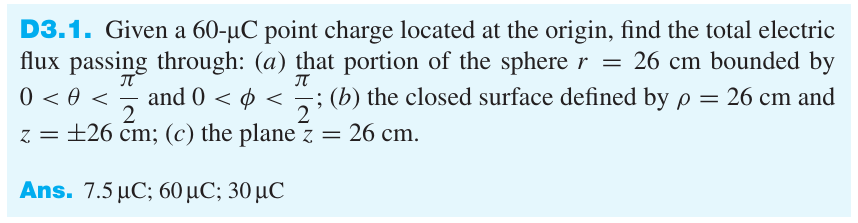
\includegraphics[width=\linewidth]{chap03/latihansoal1.png}
    \end{figure}

    \begin{itemize}
        \item Seperti yang telah diketahui bahwa kerapatan fluks adalah muatan per luasan, sehingga
        \begin{equation*}
            D = \frac{60 \times 10^{-6}}{4 \pi (26 \times 10^{-2})^2} = 7,06 \times 10^{-5} C/m^2
        \end{equation*}
        \item Selanjutnya total muatan dalam suatu area tertentu di $r = 26 cm$, $\theta$ dari $0$ hingga $\pi / 2$ dan $\phi$ dari $0$ hingga $\pi /2 $, adalah
        \begin{equation*}
            Q = \int_0^{\pi / 2} \int_0^{\pi / 2} r^2 \sin(\theta) d\theta d\phi = 0.106 m^2
        \end{equation*}
    \end{itemize}
\end{frame}

\end{document}

